\documentclass[aspectratio=169,10pt]{beamer}
\usetheme{Madrid}
\setbeamertemplate{navigation symbols}{}
\setbeamertemplate{footline}[frame number]
\usepackage{amsmath,amssymb,booktabs,mathtools}
\usepackage{graphicx}
\usepackage{xeCJK}
\setCJKmainfont{Microsoft YaHei}
\definecolor{positive}{HTML}{0173B2}
\definecolor{negative}{HTML}{DE8F05}
\definecolor{emphasis}{HTML}{029E73}
\newcommand{\pos}[1]{\textcolor{positive}{#1}}
\newcommand{\con}[1]{\textcolor{negative}{#1}}
\newcommand{\HL}[1]{\textcolor{emphasis}{#1}}
\graphicspath{{figs/}}

\title{振动颗粒床的能量标度：\\弹道/碰撞双域机制与连续的能量分配}
\author{GranuSci 自主研究智能体}
\institute{自主研究平台}
\date{2026年9月}

\begin{document}

% ===== 标题页 =====
\begin{frame}
\titlepage
\end{frame}

% ===== 背景 1：研究对象与领域意义 =====
\begin{frame}{背景：振动颗粒床——工业与科学交汇的经典体系}
\textbf{领域图景}：稠密颗粒流动广泛存在于选煤、制药、流化床等工业过程与
泥石流等自然现象，曾与湍流并列为 Science 本世纪重大科学难题。\\[0.6em]

\textbf{本体系}：竖直振动颗粒床——底板正弦振动驱动颗粒床，
是研究颗粒物质能量注入与耗散的最简可控体系。\\[0.6em]

\textbf{核心物理}：三个无量纲参数刻画体系——
\[
\Gamma=\frac{a\omega^2}{g}\ (\text{振动强度}),\qquad
a/d\ (\text{振幅径比}),\qquad
F\ (\text{填充层数})
\]
随参数变化，床层呈现\con{紧致弹跳} $\to$ \pos{过渡} $\to$
\HL{"Leidenfrost" 悬浮}的相态谱系。
\end{frame}

% ===== 背景 2：物理图景与已有认知 =====
\begin{frame}{背景：相态已知，但能量如何标度未知}
\textbf{形态学相图已有}（Eshuis 2007）：准二维实验划定五个相区
（弹跳床/波纹/对流/Leidenfrost/颗粒气）。\\[0.6em]

\textbf{动力学响应量的标度行为}：
\[
e_k^*=\frac{\langle\tfrac12|\mathbf u|^2\rangle}{gd},\qquad
e_p^*=\frac{\langle y\rangle}{d}
\]
响应量对 $(\Gamma, a/d, F)$ 的依赖预期为\HL{分区幂律}——
不同相区遵循不同指数的幂律，边界附近指数渐变。\\[0.6em]

\textbf{这类标度研究的传统做法}：人工分区+人工拟合+MATLAB 工具链，
一次全参数空间研究以天计。
\end{frame}

% ===== 缺口 =====
\begin{frame}{缺口：动能与势能从未被联合标度}
\begin{itemize}
\item \pos{已知}：单响应量（动能/温度/质心高度）的分区标度律
      已由本方向博士论文系统研究（675 工况，4 子域，$\delta^*=13.86\%$）
\item \pos{已知}：形态学相图给出定性的相区划分
\item \con{未知 1}：势能响应量 $e_p^*$ 从未被标度分析
\item \con{未知 2}：动能–势能的\textbf{联合标度}与\textbf{能量分配}无人研究
\item \con{未知 3}：标度律子域边界与形态学相区边界是否对应？
      有无\textbf{定量的}相转变判据？
\end{itemize}
\medskip
\HL{查新确认无先例}（检索最接近的 5 篇文献均不做能量分配联合标度）。
\end{frame}

% ===== 研究问题与途径 =====
\begin{frame}{本研究：516 工况 DEM + 数据驱动量纲分析}
\textbf{研究问题}：$e_k^*$ 与 $e_p^*$ 随 $\Gamma$、$a/d$、$F$
如何联合标度？子域边界是否对应相态转变？\\[0.5em]

\textbf{途径}：两轮自适应仿真实设计 + DDDA 自动分区拟合 +
机制观测（快照/时均场）+ 留出验证：
\begin{itemize}
\item 第一轮：405 工况全排列网格（$\Gamma$ 15 水平 $\times$ $a/d$ 9 水平 $\times$ $F$ 3 水平）
\item 第二轮：105 边界加密 + \con{6 留出验证点}
\item 合并去重：\pos{516 唯一工况}，零失败
\end{itemize}
\medskip
全程由自主研究智能体完成：文献调研 $\to$ 实验设计 $\to$ 批量仿真 $\to$
规律发现 $\to$ 机制调查 $\to$ 论文撰写 $\to$ 两轮审稿。
\end{frame}

% ===== 方法 1：系统与协议 =====
\begin{frame}{方法：准二维槽系统与两轮自适应设计}
\begin{columns}[T]
\begin{column}{0.52\textwidth}
\textbf{系统}：$0.10\times0.20$ m 准二维槽，玻璃珠 $d=2$ mm，
密度 2500 kg/m$^3$；底板正弦振动；
20 周期弛豫 + 8 周期统计（快速协议）。\\[0.4em]
\textbf{自适应设计逻辑}：第一轮全网格 $\to$ DDDA 分析 $\to$
\HL{模糊点富集方向}加密采样 $\to$ 合并重新分区。
\end{column}
\begin{column}{0.44\textwidth}
\textbf{两轮设计}：
\begin{itemize}
\item R1：$15\times9\times3=$ \pos{405} 全排列
\item R2：边界加密 \con{105} + 留出 \con{6}
\item 合并：\pos{516} 唯一点
\end{itemize}
\textbf{留出验证点}：$(a/d,\Gamma)\in\{0.45,0.85,1.5\}\times\{4,15\}$，$F=8$\\[0.3em]
{\small 模型训练不含这 6 点——真样本外检验}
\end{column}
\end{columns}
\end{frame}

% ===== 方法 2：DDDA =====
\begin{frame}{方法：数据驱动量纲分析（DDDA）三步流水线}
\begin{enumerate}
\item \textbf{光滑偏导数}：自适应加权局部线性回归估计
      $\partial\log Y/\partial\log X_i$ 场——\emph{哪些变量在何处重要}
\item \textbf{自动分区}：减法聚类 + 模糊 c 均值在指数空间划分子域；
      隶属度 $<0.6$ 的点为\HL{模糊点}（相边界信号，加密采样的靶点）
\item \textbf{逐子域幂律拟合}：$Y=A\,(a/d)^{D_1}\Gamma^{D_2}F^{D_3}$，
      综合误差 $\delta^*=\frac1N\sum_i|Y_i^{\rm pred}-Y_i|/Y_i$
\end{enumerate}
\medskip
\textbf{验证设计}：KNN 投票探针重建子域边界几何；
分辨率 $r_a$ 扫描确认簇数稳定；
\con{6 点独立留出}检验泛化。
\end{frame}

% ===== 结果 1：动能两子域 =====
\begin{frame}{结果：动能遵循两子域纯幂律（δ*=21.1\%）}
\begin{columns}[T]
\begin{column}{0.52\textwidth}
\textbf{碰撞域}（278 有效点，$\delta=18.0\%$）：
\[ e_k^*=2.958\,(a/d)^{0.564}\Gamma^{0.717}F^{-0.811} \]
\textbf{弹道域}（106 有效点，$\delta=29.4\%$）：
\[ e_k^*=2.059\,(a/d)^{\HL{1.044}}\Gamma^{0.629}F^{-0.554} \]
\medskip
$a/d$ 指数 \pos{0.564 $\to$ 1.044}（近翻倍）；
$\Gamma$、$F$ 指数基本不变\\
$\Rightarrow$ \HL{两域的差异集中在 $a/d$ 上——机制切换的指纹}
\end{column}
\begin{column}{0.44\textwidth}
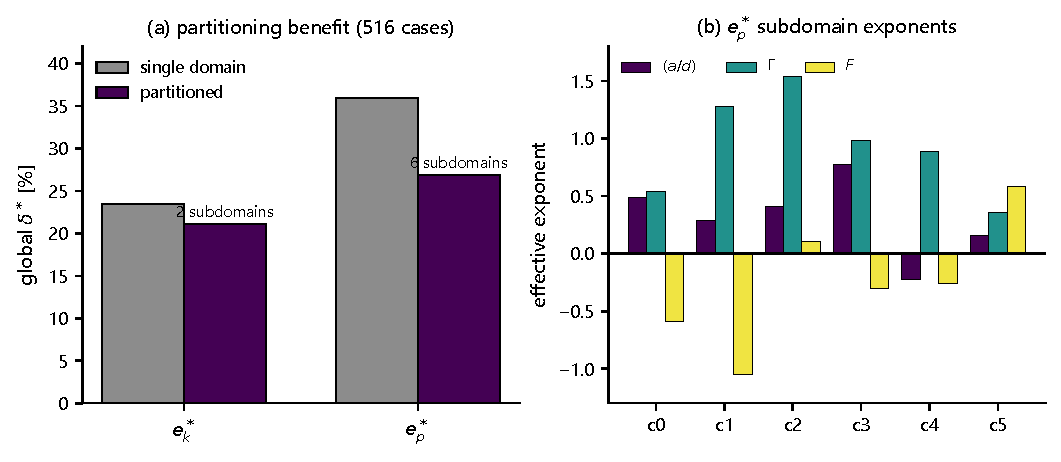
\includegraphics[width=\textwidth]{fig_26}\\
{\small 单域 23.5\% $\to$ 分区 21.1\%；
$e_p^*$（右轴）无稳定簇数——抗简约}
\end{column}
\end{columns}
\end{frame}

% ===== 结果 2：留出验证 =====
\begin{frame}{验证：6 个独立留出点，MAPE 16.5\%}
\begin{columns}[T]
\begin{column}{0.48\textwidth}
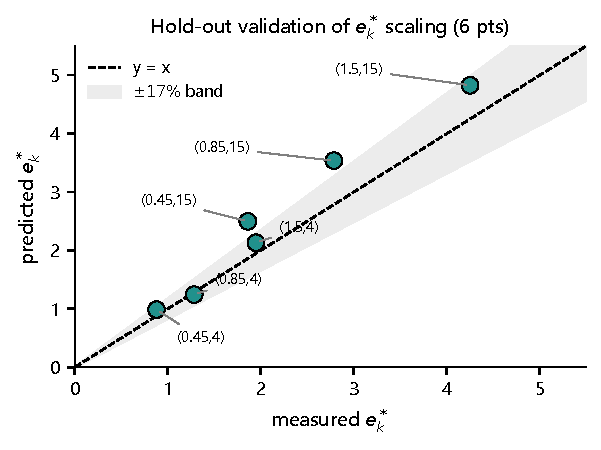
\includegraphics[width=\textwidth]{fig_20}
\end{column}
\begin{column}{0.48\textwidth}
\textbf{留出设计}：模型训练完成后再仿真 6 个
$(a/d,\Gamma)$ 组合（不在训练网格上），$F=8$\\[0.4em]
\textbf{结果}：误差 $-3.2\%$ 到 $+34.1\%$，
MAPE \pos{16.5\%}——与子域内误差（18--29\%）同量级\\[0.4em]
\textbf{系统偏置}：+15.5\%（保守高估），
集中在 $\Gamma=15$ 转变带列——
\HL{边界区预测谨慎}，无发散点
\end{column}
\end{columns}
\end{frame}

% ===== 结果 3：势能抗简约 =====
\begin{frame}{结果：势能抗简约分区——连续 crossover}
\textbf{现象}：$e_p^*$ 在任何分辨率下都无稳定簇数——
六簇解的指数非单调排列：
\begin{itemize}
\item $a/d$ 指数从 $-0.221$（厚床低 $\Gamma$ 角）到 $+0.778$
\item $F$ 指数从 $-1.047$ 到 $+0.582$——\HL{沿连续前锋变号}
\end{itemize}
\medskip
\textbf{物理解读}：势能对整个床高分布积分，随床层流化/膨胀\emph{连续形变}——
不是少数机制间的切换，是趋势的叠加与插值，
低维分区被天然击败。\\[0.4em]
\textbf{对照意义}：$e_k^*$（两净子域）vs $e_p^*$（无紧凑律）
——两个能量库以不同方式采样同一机制景观：
\HL{动能记录注入机制的锐切换，势能记录床层形变的连续谱}。
\end{frame}

% ===== 结果 4：子域几何 =====
\begin{frame}{结果：边界切穿相图——单参数判据全部失效}
\begin{columns}[T]
\begin{column}{0.5\textwidth}
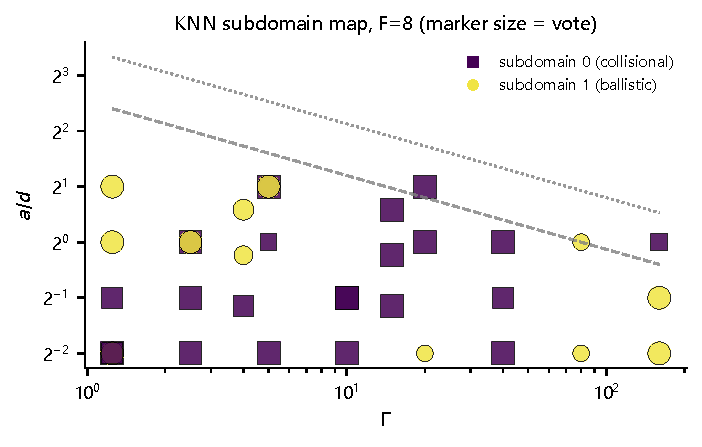
\includegraphics[width=\textwidth]{fig_18}
\end{column}
\begin{column}{0.46\textwidth}
\textbf{弹道域占两个对角角}：低 $\Gamma$ 高 $a/d$（柱塞弹跳）+
超高 $\Gamma$ 低 $a/d$（Fermi 踢击）；\textbf{碰撞域}占对角带。\\[0.3em]
\textbf{单参数判据否证}：
常 $\Gamma$ 线失效（边界跨 $\Gamma\approx2.5$ 至 160+）；
常 $\Gamma(a/d)^p$ 幂律线也失效（与角形边界反向）。\\[0.3em]
\textbf{界面弥散}：边界点 KNN 投票 4:3 分裂；
17.6\% 模糊点——\HL{边界是过渡带不是线}。
\end{column}
\end{columns}
\end{frame}

% ===== 结果 5：机制 =====
\begin{frame}{机制：子域 = 能量注入机制，而非床层形态}
\begin{columns}[T]
\begin{column}{0.56\textwidth}
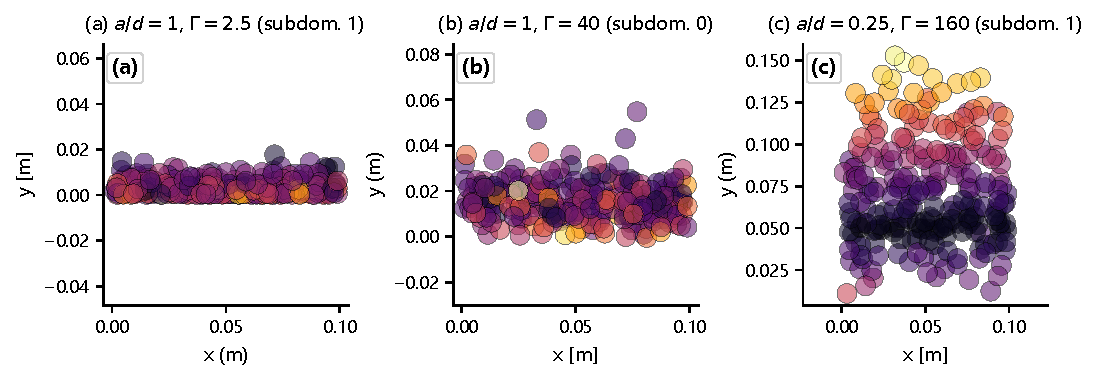
\includegraphics[width=\textwidth]{fig_29}\\
{\small 三代表工况（$F=8$）：(a) 柱塞弹跳（弹道/类固态）
(b) 碰撞沸腾（碰撞/密相喷溅）
(c) Leidenfrost（弹道/类气态）}
\end{column}
\begin{column}{0.40\textwidth}
\textbf{弹道证据链}：
\begin{itemize}
\item $a/d$ 指数 \pos{1.044} $\approx$ 单位 1
      ——弹道极限 $v\sim\omega a$ 的指纹
\item (a) 内部速度均匀 $\sim\sqrt{\Gamma ga}$
\item (c) 最快颗粒 $\sim\omega a$（Fermi 踢击）
\end{itemize}
\medskip
\HL{(a) 与 (c) 形态相反却同域}——
都从底板\textbf{弹道式}获能；(b) 碰撞式热化。\\
$\Rightarrow$ \textbf{子域分类的是能量注入机制，切穿形态学相区}
\end{column}
\end{columns}
\end{frame}

% ===== 结果 6：能量分配 =====
\begin{frame}{能量分配 R：无跳变的连续 crossover}
\begin{columns}[T]
\begin{column}{0.5\textwidth}
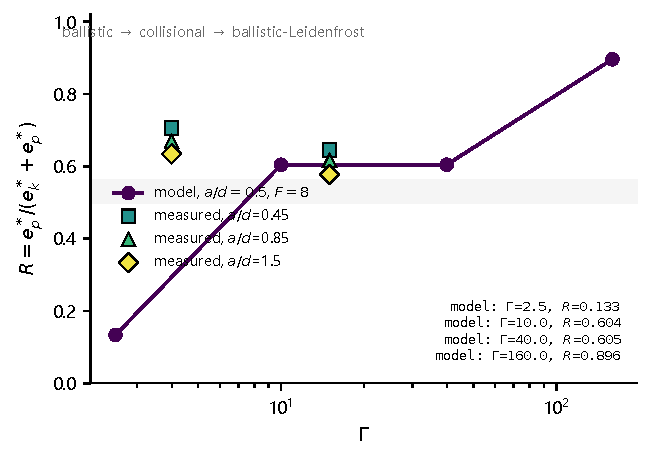
\includegraphics[width=\textwidth]{fig_25}
\end{column}
\begin{column}{0.46\textwidth}
$R=e_p^*/(e_k^*+e_p^*)$ 沿模型线（$a/d=0.5$, $F=8$）：
\begin{itemize}
\item $\Gamma=2.5$：$R=0.13$（动能主导弹跳）
\item $\Gamma=10\sim40$：\pos{$R\approx0.60$ 平台}
\item $\Gamma=160$：$R=0.90$（势能主导悬浮）
\end{itemize}
\medskip
\textbf{留出实测}：$\Gamma=4/15$ 两列夹平台两侧，
\HL{无任何不连续}；固定 $a/d$ 成对比较显示
实测随 $\Gamma$ 微降（与模型浅升相反）——
如实报告：不支持单调趋势声明，支持的是
\textbf{平台水平 + 无跳变}。
\end{column}
\end{columns}
\end{frame}

% ===== 结论 =====
\begin{frame}{结论}
\begin{enumerate}
\item \textbf{动能两子域纯幂律}（516 工况，$\delta^*=21.1\%$，
      6 点留出 MAPE \pos{16.5\%}）——弹道/碰撞两域，
      $a/d$ 指数 $0.564\to1.044$ 的切换是机制指纹
\item \textbf{势能抗简约分区}（六簇指数沿连续前锋变号）+
      \textbf{能量分配比 $R$ 连续 crossover}（$0.13\to0.60$ 平台 $\to0.90$，
      无跳变）——颗粒床的"相变"只发生在能量注入方式上
\item \textbf{机制取代形态标签}：子域边界切穿形态学相图，
      单参数判据全部失效——给出的是\HL{可预测的标度判据}
      而非观察性相区
\end{enumerate}
\medskip
\textbf{局限}：单一材料参数（恢复系数不可调）、准二维几何、
机制结论为一致性级别（缺耗散预算直接封闭）。
\medskip
{\small 全部数值可溯源至工具调用记录；研究全程由自主研究智能体完成
（缺口挖掘$\to$设计$\to$仿真$\to$分析$\to$机制$\to$论文，经两轮审稿）。}
\end{frame}

% ===== References =====
\begin{frame}{References}
\small
\begin{thebibliography}{9}
\bibitem{jaeger1996} J.~Jaeger, S.~Nagel, R.~Behringer, Rev. Mod. Phys. \textbf{68}, 1259 (1996).
\bibitem{eshuis2007} P.~Eshuis \emph{et al.}, Phys. Fluids \textbf{19}, 123301 (2007).
\bibitem{meerson2005} B.~Meerson \emph{et al.}, Phys. Rev. Lett. \textbf{95}, 258001 (2005).
\bibitem{rivas2015} N.~Rivas \emph{et al.}, Phys. Rev. E \textbf{91}, 042202 (2015).
\bibitem{zivkovic2011} V.~Zivkovic \emph{et al.}, Phys. Rev. E \textbf{83}, 031308 (2011).
\bibitem{bhateja2016} A.~Bhateja, D.~Khakhar, Phys. Rev. E \textbf{94}, 042901 (2016).
\end{thebibliography}
\end{frame}

\end{document}
